% !TEX TS-program = pdflatex
% !TEX encoding = UTF-8 Unicode
\documentclass[border=0mm]{standalone}
% packages
\usepackage{tikz}
\usetikzlibrary{patterns}
\usepackage{amsmath,amssymb}
\usepackage{bm}
\usepackage{pgfplots}
\pgfplotsset{compat=1.15}
% start document
\begin{document}
% generated by ROOT (CERN)
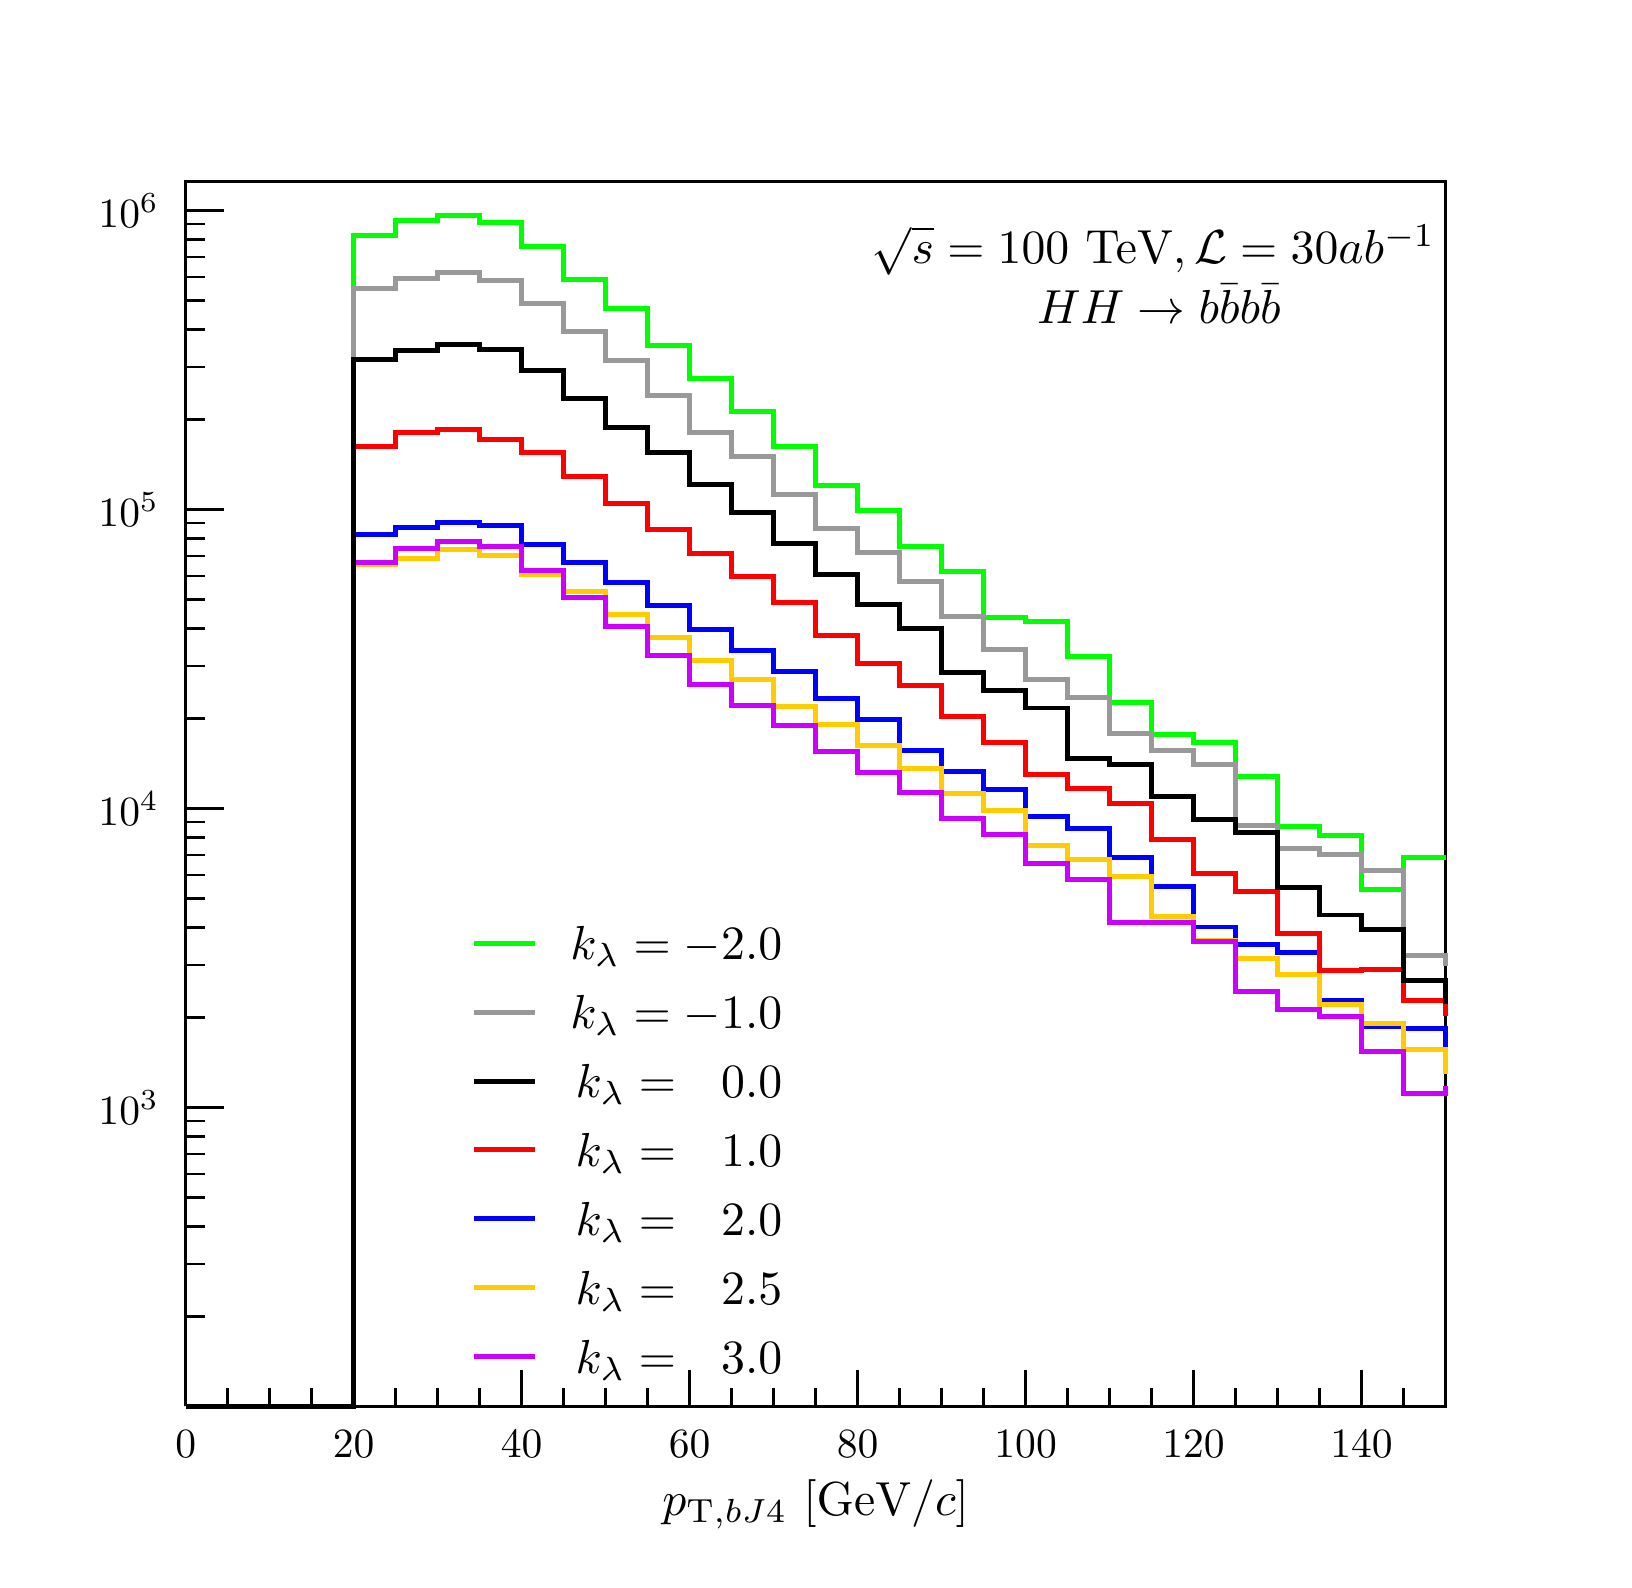
\begin{tikzpicture}
\pgfdeclareplotmark{cross} {
\pgfpathmoveto{\pgfpoint{-0.3\pgfplotmarksize}{\pgfplotmarksize}}
\pgfpathlineto{\pgfpoint{+0.3\pgfplotmarksize}{\pgfplotmarksize}}
\pgfpathlineto{\pgfpoint{+0.3\pgfplotmarksize}{0.3\pgfplotmarksize}}
\pgfpathlineto{\pgfpoint{+1\pgfplotmarksize}{0.3\pgfplotmarksize}}
\pgfpathlineto{\pgfpoint{+1\pgfplotmarksize}{-0.3\pgfplotmarksize}}
\pgfpathlineto{\pgfpoint{+0.3\pgfplotmarksize}{-0.3\pgfplotmarksize}}
\pgfpathlineto{\pgfpoint{+0.3\pgfplotmarksize}{-1.\pgfplotmarksize}}
\pgfpathlineto{\pgfpoint{-0.3\pgfplotmarksize}{-1.\pgfplotmarksize}}
\pgfpathlineto{\pgfpoint{-0.3\pgfplotmarksize}{-0.3\pgfplotmarksize}}
\pgfpathlineto{\pgfpoint{-1.\pgfplotmarksize}{-0.3\pgfplotmarksize}}
\pgfpathlineto{\pgfpoint{-1.\pgfplotmarksize}{0.3\pgfplotmarksize}}
\pgfpathlineto{\pgfpoint{-0.3\pgfplotmarksize}{0.3\pgfplotmarksize}}
\pgfpathclose
\pgfusepathqstroke
}
\pgfdeclareplotmark{cross*} {
\pgfpathmoveto{\pgfpoint{-0.3\pgfplotmarksize}{\pgfplotmarksize}}
\pgfpathlineto{\pgfpoint{+0.3\pgfplotmarksize}{\pgfplotmarksize}}
\pgfpathlineto{\pgfpoint{+0.3\pgfplotmarksize}{0.3\pgfplotmarksize}}
\pgfpathlineto{\pgfpoint{+1\pgfplotmarksize}{0.3\pgfplotmarksize}}
\pgfpathlineto{\pgfpoint{+1\pgfplotmarksize}{-0.3\pgfplotmarksize}}
\pgfpathlineto{\pgfpoint{+0.3\pgfplotmarksize}{-0.3\pgfplotmarksize}}
\pgfpathlineto{\pgfpoint{+0.3\pgfplotmarksize}{-1.\pgfplotmarksize}}
\pgfpathlineto{\pgfpoint{-0.3\pgfplotmarksize}{-1.\pgfplotmarksize}}
\pgfpathlineto{\pgfpoint{-0.3\pgfplotmarksize}{-0.3\pgfplotmarksize}}
\pgfpathlineto{\pgfpoint{-1.\pgfplotmarksize}{-0.3\pgfplotmarksize}}
\pgfpathlineto{\pgfpoint{-1.\pgfplotmarksize}{0.3\pgfplotmarksize}}
\pgfpathlineto{\pgfpoint{-0.3\pgfplotmarksize}{0.3\pgfplotmarksize}}
\pgfpathclose
\pgfusepathqfillstroke
}
\pgfdeclareplotmark{newstar} {
\pgfpathmoveto{\pgfqpoint{0pt}{\pgfplotmarksize}}
\pgfpathlineto{\pgfqpointpolar{44}{0.5\pgfplotmarksize}}
\pgfpathlineto{\pgfqpointpolar{18}{\pgfplotmarksize}}
\pgfpathlineto{\pgfqpointpolar{-20}{0.5\pgfplotmarksize}}
\pgfpathlineto{\pgfqpointpolar{-54}{\pgfplotmarksize}}
\pgfpathlineto{\pgfqpointpolar{-90}{0.5\pgfplotmarksize}}
\pgfpathlineto{\pgfqpointpolar{234}{\pgfplotmarksize}}
\pgfpathlineto{\pgfqpointpolar{198}{0.5\pgfplotmarksize}}
\pgfpathlineto{\pgfqpointpolar{162}{\pgfplotmarksize}}
\pgfpathlineto{\pgfqpointpolar{134}{0.5\pgfplotmarksize}}
\pgfpathclose
\pgfusepathqstroke
}
\pgfdeclareplotmark{newstar*} {
\pgfpathmoveto{\pgfqpoint{0pt}{\pgfplotmarksize}}
\pgfpathlineto{\pgfqpointpolar{44}{0.5\pgfplotmarksize}}
\pgfpathlineto{\pgfqpointpolar{18}{\pgfplotmarksize}}
\pgfpathlineto{\pgfqpointpolar{-20}{0.5\pgfplotmarksize}}
\pgfpathlineto{\pgfqpointpolar{-54}{\pgfplotmarksize}}
\pgfpathlineto{\pgfqpointpolar{-90}{0.5\pgfplotmarksize}}
\pgfpathlineto{\pgfqpointpolar{234}{\pgfplotmarksize}}
\pgfpathlineto{\pgfqpointpolar{198}{0.5\pgfplotmarksize}}
\pgfpathlineto{\pgfqpointpolar{162}{\pgfplotmarksize}}
\pgfpathlineto{\pgfqpointpolar{134}{0.5\pgfplotmarksize}}
\pgfpathclose
\pgfusepathqfillstroke
}
\definecolor{c}{rgb}{1,1,1};
\draw [color=c, fill=c] (0,0) rectangle (20,19.4486);
\draw [color=c, fill=c] (0,0) rectangle (20,19.4486);
\draw [color=c, fill=c] (2,1.94486) rectangle (18,17.5038);
\definecolor{c}{rgb}{0,0,0};
\draw [c,line width=0.9] (2,1.94486) -- (2,17.5038) -- (18,17.5038) -- (18,1.94486) -- (2,1.94486);
\definecolor{c}{rgb}{1,1,1};
\draw [color=c, fill=c] (2,1.94486) rectangle (18,17.5038);
\definecolor{c}{rgb}{0,0,0};
\draw [c,line width=0.9] (2,1.94486) -- (2,17.5038) -- (18,17.5038) -- (18,1.94486) -- (2,1.94486);
\definecolor{c}{rgb}{0,1,0};
\draw [c,line width=1.8] (2,1.94486) -- (2.53333,1.94486) -- (2.53333,1.94486) -- (3.06667,1.94486) -- (3.06667,1.94486) -- (3.6,1.94486) -- (3.6,1.94486) -- (4.13333,1.94486) -- (4.13333,16.8121) -- (4.66667,16.8121) -- (4.66667,17.0019) --
 (5.2,17.0019) -- (5.2,17.0711) -- (5.73333,17.0711) -- (5.73333,16.9835) -- (6.26667,16.9835) -- (6.26667,16.6729) -- (6.8,16.6729) -- (6.8,16.2588) -- (7.33333,16.2588) -- (7.33333,15.8869) -- (7.86667,15.8869) -- (7.86667,15.4159) -- (8.4,15.4159)
 -- (8.4,14.9968) -- (8.93333,14.9968) -- (8.93333,14.5751) -- (9.46667,14.5751) -- (9.46667,14.1358) -- (10,14.1358) -- (10,13.6445) -- (10.5333,13.6445) -- (10.5333,13.324) -- (11.0667,13.324) -- (11.0667,12.8722) -- (11.6,12.8722) --
 (11.6,12.5518) -- (12.1333,12.5518) -- (12.1333,11.967) -- (12.6667,11.967) -- (12.6667,11.9095) -- (13.2,11.9095) -- (13.2,11.4641) -- (13.7333,11.4641) -- (13.7333,10.8796) -- (14.2667,10.8796) -- (14.2667,10.4794) -- (14.8,10.4794) --
 (14.8,10.3714) -- (15.3333,10.3714) -- (15.3333,9.94993) -- (15.8667,9.94993) -- (15.8667,9.31304) -- (16.4,9.31304) -- (16.4,9.19083) -- (16.9333,9.19083) -- (16.9333,8.50949) -- (17.4667,8.50949) -- (17.4667,8.91537) -- (18,8.91537);
\definecolor{c}{rgb}{0,0,0};
\draw [c,line width=0.9] (2,1.94486) -- (18,1.94486);
\draw [c,line width=0.9] (2,2.41163) -- (2,1.94486);
\draw [c,line width=0.9] (2.53333,2.17825) -- (2.53333,1.94486);
\draw [c,line width=0.9] (3.06667,2.17825) -- (3.06667,1.94486);
\draw [c,line width=0.9] (3.6,2.17825) -- (3.6,1.94486);
\draw [c,line width=0.9] (4.13333,2.41163) -- (4.13333,1.94486);
\draw [c,line width=0.9] (4.66667,2.17825) -- (4.66667,1.94486);
\draw [c,line width=0.9] (5.2,2.17825) -- (5.2,1.94486);
\draw [c,line width=0.9] (5.73333,2.17825) -- (5.73333,1.94486);
\draw [c,line width=0.9] (6.26667,2.41163) -- (6.26667,1.94486);
\draw [c,line width=0.9] (6.8,2.17825) -- (6.8,1.94486);
\draw [c,line width=0.9] (7.33333,2.17825) -- (7.33333,1.94486);
\draw [c,line width=0.9] (7.86667,2.17825) -- (7.86667,1.94486);
\draw [c,line width=0.9] (8.4,2.41163) -- (8.4,1.94486);
\draw [c,line width=0.9] (8.93333,2.17825) -- (8.93333,1.94486);
\draw [c,line width=0.9] (9.46667,2.17825) -- (9.46667,1.94486);
\draw [c,line width=0.9] (10,2.17825) -- (10,1.94486);
\draw [c,line width=0.9] (10.5333,2.41163) -- (10.5333,1.94486);
\draw [c,line width=0.9] (11.0667,2.17825) -- (11.0667,1.94486);
\draw [c,line width=0.9] (11.6,2.17825) -- (11.6,1.94486);
\draw [c,line width=0.9] (12.1333,2.17825) -- (12.1333,1.94486);
\draw [c,line width=0.9] (12.6667,2.41163) -- (12.6667,1.94486);
\draw [c,line width=0.9] (13.2,2.17825) -- (13.2,1.94486);
\draw [c,line width=0.9] (13.7333,2.17825) -- (13.7333,1.94486);
\draw [c,line width=0.9] (14.2667,2.17825) -- (14.2667,1.94486);
\draw [c,line width=0.9] (14.8,2.41163) -- (14.8,1.94486);
\draw [c,line width=0.9] (15.3333,2.17825) -- (15.3333,1.94486);
\draw [c,line width=0.9] (15.8667,2.17825) -- (15.8667,1.94486);
\draw [c,line width=0.9] (16.4,2.17825) -- (16.4,1.94486);
\draw [c,line width=0.9] (16.9333,2.41163) -- (16.9333,1.94486);
\draw [c,line width=0.9] (16.9333,2.41163) -- (16.9333,1.94486);
\draw [c,line width=0.9] (17.4667,2.17825) -- (17.4667,1.94486);
\draw [c,line width=0.9] (18,2.17825) -- (18,1.94486);
\draw [anchor=base] (2,1.30306) node[scale=1.50291, color=c, rotate=0]{0};
\draw [anchor=base] (4.13333,1.30306) node[scale=1.50291, color=c, rotate=0]{20};
\draw [anchor=base] (6.26667,1.30306) node[scale=1.50291, color=c, rotate=0]{40};
\draw [anchor=base] (8.4,1.30306) node[scale=1.50291, color=c, rotate=0]{60};
\draw [anchor=base] (10.5333,1.30306) node[scale=1.50291, color=c, rotate=0]{80};
\draw [anchor=base] (12.6667,1.30306) node[scale=1.50291, color=c, rotate=0]{100};
\draw [anchor=base] (14.8,1.30306) node[scale=1.50291, color=c, rotate=0]{120};
\draw [anchor=base] (16.9333,1.30306) node[scale=1.50291, color=c, rotate=0]{140};
\draw (10,0.700151) node[scale=1.72557, color=c, rotate=0]{$p_{\text{T}, bJ4} ~[\text{GeV}/c]$};
\draw [c,line width=0.9] (2,1.94486) -- (2,17.5038);
\draw [c,line width=0.9] (2.24,3.08785) -- (2,3.08785);
\draw [c,line width=0.9] (2.24,3.75646) -- (2,3.75646);
\draw [c,line width=0.9] (2.24,4.23084) -- (2,4.23084);
\draw [c,line width=0.9] (2.24,4.5988) -- (2,4.5988);
\draw [c,line width=0.9] (2.24,4.89945) -- (2,4.89945);
\draw [c,line width=0.9] (2.24,5.15364) -- (2,5.15364);
\draw [c,line width=0.9] (2.24,5.37383) -- (2,5.37383);
\draw [c,line width=0.9] (2.24,5.56806) -- (2,5.56806);
\draw [c,line width=0.9] (2.48,5.74179) -- (2,5.74179);
\draw [anchor= east] (1.844,5.74179) node[scale=1.50291, color=c, rotate=0]{$10^{3}$};
\draw [c,line width=0.9] (2.24,6.88479) -- (2,6.88479);
\draw [c,line width=0.9] (2.24,7.55339) -- (2,7.55339);
\draw [c,line width=0.9] (2.24,8.02778) -- (2,8.02778);
\draw [c,line width=0.9] (2.24,8.39574) -- (2,8.39574);
\draw [c,line width=0.9] (2.24,8.69638) -- (2,8.69638);
\draw [c,line width=0.9] (2.24,8.95058) -- (2,8.95058);
\draw [c,line width=0.9] (2.24,9.17077) -- (2,9.17077);
\draw [c,line width=0.9] (2.24,9.36499) -- (2,9.36499);
\draw [c,line width=0.9] (2.48,9.53873) -- (2,9.53873);
\draw [anchor= east] (1.844,9.53873) node[scale=1.50291, color=c, rotate=0]{$10^{4}$};
\draw [c,line width=0.9] (2.24,10.6817) -- (2,10.6817);
\draw [c,line width=0.9] (2.24,11.3503) -- (2,11.3503);
\draw [c,line width=0.9] (2.24,11.8247) -- (2,11.8247);
\draw [c,line width=0.9] (2.24,12.1927) -- (2,12.1927);
\draw [c,line width=0.9] (2.24,12.4933) -- (2,12.4933);
\draw [c,line width=0.9] (2.24,12.7475) -- (2,12.7475);
\draw [c,line width=0.9] (2.24,12.9677) -- (2,12.9677);
\draw [c,line width=0.9] (2.24,13.1619) -- (2,13.1619);
\draw [c,line width=0.9] (2.48,13.3357) -- (2,13.3357);
\draw [anchor= east] (1.844,13.3357) node[scale=1.50291, color=c, rotate=0]{$10^{5}$};
\draw [c,line width=0.9] (2.24,14.4787) -- (2,14.4787);
\draw [c,line width=0.9] (2.24,15.1473) -- (2,15.1473);
\draw [c,line width=0.9] (2.24,15.6216) -- (2,15.6216);
\draw [c,line width=0.9] (2.24,15.9896) -- (2,15.9896);
\draw [c,line width=0.9] (2.24,16.2903) -- (2,16.2903);
\draw [c,line width=0.9] (2.24,16.5444) -- (2,16.5444);
\draw [c,line width=0.9] (2.24,16.7646) -- (2,16.7646);
\draw [c,line width=0.9] (2.24,16.9589) -- (2,16.9589);
\draw [c,line width=0.9] (2.48,17.1326) -- (2,17.1326);
\draw [anchor= east] (1.844,17.1326) node[scale=1.50291, color=c, rotate=0]{$10^{6}$};
\definecolor{c}{rgb}{0,0,1};
\draw [c,line width=1.8] (2,1.94486) -- (2.53333,1.94486) -- (2.53333,1.94486) -- (3.06667,1.94486) -- (3.06667,1.94486) -- (3.6,1.94486) -- (3.6,1.94486) -- (4.13333,1.94486) -- (4.13333,13.0208) -- (4.66667,13.0208) -- (4.66667,13.1072) --
 (5.2,13.1072) -- (5.2,13.1694) -- (5.73333,13.1694) -- (5.73333,13.1276) -- (6.26667,13.1276) -- (6.26667,12.8892) -- (6.8,12.8892) -- (6.8,12.6675) -- (7.33333,12.6675) -- (7.33333,12.4036) -- (7.86667,12.4036) -- (7.86667,12.1217) -- (8.4,12.1217)
 -- (8.4,11.8075) -- (8.93333,11.8075) -- (8.93333,11.5397) -- (9.46667,11.5397) -- (9.46667,11.273) -- (10,11.273) -- (10,10.9315) -- (10.5333,10.9315) -- (10.5333,10.6672) -- (11.0667,10.6672) -- (11.0667,10.2794) -- (11.6,10.2794) --
 (11.6,10.0132) -- (12.1333,10.0132) -- (12.1333,9.77506) -- (12.6667,9.77506) -- (12.6667,9.4335) -- (13.2,9.4335) -- (13.2,9.2874) -- (13.7333,9.2874) -- (13.7333,8.91944) -- (14.2667,8.91944) -- (14.2667,8.54692) -- (14.8,8.54692) -- (14.8,8.0341)
 -- (15.3333,8.0341) -- (15.3333,7.80648) -- (15.8667,7.80648) -- (15.8667,7.70837) -- (16.4,7.70837) -- (16.4,7.1048) -- (16.9333,7.1048) -- (16.9333,6.77289) -- (17.4667,6.77289) -- (17.4667,6.75045) -- (18,6.75045) -- (18,6.17516) -- (18,6.17516);
\definecolor{c}{rgb}{1,0.8,0};
\draw [c,line width=1.8] (2,1.94486) -- (2.53333,1.94486) -- (2.53333,1.94486) -- (3.06667,1.94486) -- (3.06667,1.94486) -- (3.6,1.94486) -- (3.6,1.94486) -- (4.13333,1.94486) -- (4.13333,12.6408) -- (4.66667,12.6408) -- (4.66667,12.7172) --
 (5.2,12.7172) -- (5.2,12.828) -- (5.73333,12.828) -- (5.73333,12.7548) -- (6.26667,12.7548) -- (6.26667,12.5164) -- (6.8,12.5164) -- (6.8,12.2943) -- (7.33333,12.2943) -- (7.33333,12.0051) -- (7.86667,12.0051) -- (7.86667,11.7163) -- (8.4,11.7163)
 -- (8.4,11.4125) -- (8.93333,11.4125) -- (8.93333,11.1764) -- (9.46667,11.1764) -- (9.46667,10.8298) -- (10,10.8298) -- (10,10.6092) -- (10.5333,10.6092) -- (10.5333,10.3418) -- (11.0667,10.3418) -- (11.0667,10.0469) -- (11.6,10.0469) --
 (11.6,9.72382) -- (12.1333,9.72382) -- (12.1333,9.51295) -- (12.6667,9.51295) -- (12.6667,9.07073) -- (13.2,9.07073) -- (13.2,8.89235) -- (13.7333,8.89235) -- (13.7333,8.68062) -- (14.2667,8.68062) -- (14.2667,8.16864) -- (14.8,8.16864) --
 (14.8,7.86158) -- (15.3333,7.86158) -- (15.3333,7.64001) -- (15.8667,7.64001) -- (15.8667,7.42846) -- (16.4,7.42846) -- (16.4,7.04949) -- (16.9333,7.04949) -- (16.9333,6.8123) -- (17.4667,6.8123) -- (17.4667,6.48039) -- (18,6.48039) -- (18,6.16182)
 -- (18,6.16182);
\definecolor{c}{rgb}{0.8,0,1};
\draw [c,line width=1.8] (2,1.94486) -- (2.53333,1.94486) -- (2.53333,1.94486) -- (3.06667,1.94486) -- (3.06667,1.94486) -- (3.6,1.94486) -- (3.6,1.94486) -- (4.13333,1.94486) -- (4.13333,12.6666) -- (4.66667,12.6666) -- (4.66667,12.8454) --
 (5.2,12.8454) -- (5.2,12.9255) -- (5.73333,12.9255) -- (5.73333,12.8668) -- (6.26667,12.8668) -- (6.26667,12.5605) -- (6.8,12.5605) -- (6.8,12.2126) -- (7.33333,12.2126) -- (7.33333,11.8442) -- (7.86667,11.8442) -- (7.86667,11.485) -- (8.4,11.485)
 -- (8.4,11.1099) -- (8.93333,11.1099) -- (8.93333,10.8495) -- (9.46667,10.8495) -- (9.46667,10.5964) -- (10,10.5964) -- (10,10.2597) -- (10.5333,10.2597) -- (10.5333,9.99574) -- (11.0667,9.99574) -- (11.0667,9.74108) -- (11.6,9.74108) --
 (11.6,9.41614) -- (12.1333,9.41614) -- (12.1333,9.21371) -- (12.6667,9.21371) -- (12.6667,8.84295) -- (13.2,8.84295) -- (13.2,8.63674) -- (13.7333,8.63674) -- (13.7333,8.09522) -- (14.2667,8.09522) -- (14.2667,8.09522) -- (14.8,8.09522) --
 (14.8,7.85277) -- (15.3333,7.85277) -- (15.3333,7.21712) -- (15.8667,7.21712) -- (15.8667,6.99154) -- (16.4,6.99154) -- (16.4,6.90287) -- (16.9333,6.90287) -- (16.9333,6.45559) -- (17.4667,6.45559) -- (17.4667,5.92448) -- (18,5.92448) --
 (18,6.02056) -- (18,6.02056);
\definecolor{c}{rgb}{0.6,0.6,0.6};
\draw [c,line width=1.8] (2,1.94486) -- (2.53333,1.94486) -- (2.53333,1.94486) -- (3.06667,1.94486) -- (3.06667,1.94486) -- (3.6,1.94486) -- (3.6,1.94486) -- (4.13333,1.94486) -- (4.13333,16.1404) -- (4.66667,16.1404) -- (4.66667,16.2645) --
 (5.2,16.2645) -- (5.2,16.3417) -- (5.73333,16.3417) -- (5.73333,16.248) -- (6.26667,16.248) -- (6.26667,15.9543) -- (6.8,15.9543) -- (6.8,15.5995) -- (7.33333,15.5995) -- (7.33333,15.2344) -- (7.86667,15.2344) -- (7.86667,14.7869) -- (8.4,14.7869)
 -- (8.4,14.3173) -- (8.93333,14.3173) -- (8.93333,14.0068) -- (9.46667,14.0068) -- (9.46667,13.5251) -- (10,13.5251) -- (10,13.0986) -- (10.5333,13.0986) -- (10.5333,12.7905) -- (11.0667,12.7905) -- (11.0667,12.4184) -- (11.6,12.4184) --
 (11.6,11.9739) -- (12.1333,11.9739) -- (12.1333,11.5621) -- (12.6667,11.5621) -- (12.6667,11.1775) -- (13.2,11.1775) -- (13.2,10.9509) -- (13.7333,10.9509) -- (13.7333,10.4916) -- (14.2667,10.4916) -- (14.2667,10.2767) -- (14.8,10.2767) --
 (14.8,10.0973) -- (15.3333,10.0973) -- (15.3333,9.32602) -- (15.8667,9.32602) -- (15.8667,9.0284) -- (16.4,9.0284) -- (16.4,8.95427) -- (16.9333,8.95427) -- (16.9333,8.75293) -- (17.4667,8.75293) -- (17.4667,7.67296) -- (18,7.67296) -- (18,7.54441)
 -- (18,7.54441);
\definecolor{c}{rgb}{1,0,0};
\draw [c,line width=1.8] (2,1.94486) -- (2.53333,1.94486) -- (2.53333,1.94486) -- (3.06667,1.94486) -- (3.06667,1.94486) -- (3.6,1.94486) -- (3.6,1.94486) -- (4.13333,1.94486) -- (4.13333,14.1303) -- (4.66667,14.1303) -- (4.66667,14.3083) --
 (5.2,14.3083) -- (5.2,14.3483) -- (5.73333,14.3483) -- (5.73333,14.223) -- (6.26667,14.223) -- (6.26667,14.0631) -- (6.8,14.0631) -- (6.8,13.7573) -- (7.33333,13.7573) -- (7.33333,13.4106) -- (7.86667,13.4106) -- (7.86667,13.0865) -- (8.4,13.0865)
 -- (8.4,12.7784) -- (8.93333,12.7784) -- (8.93333,12.4834) -- (9.46667,12.4834) -- (9.46667,12.159) -- (10,12.159) -- (10,11.7303) -- (10.5333,11.7303) -- (10.5333,11.3795) -- (11.0667,11.3795) -- (11.0667,11.1043) -- (11.6,11.1043) --
 (11.6,10.7129) -- (12.1333,10.7129) -- (12.1333,10.3771) -- (12.6667,10.3771) -- (12.6667,9.97386) -- (13.2,9.97386) -- (13.2,9.79908) -- (13.7333,9.79908) -- (13.7333,9.59963) -- (14.2667,9.59963) -- (14.2667,9.14605) -- (14.8,9.14605) --
 (14.8,8.71754) -- (15.3333,8.71754) -- (15.3333,8.48775) -- (15.8667,8.48775) -- (15.8667,7.95587) -- (16.4,7.95587) -- (16.4,7.47793) -- (16.9333,7.47793) -- (16.9333,7.49209) -- (17.4667,7.49209) -- (17.4667,7.09569) -- (18,7.09569) --
 (18,6.90595) -- (18,6.90595);
\definecolor{c}{rgb}{0,0,0};
\draw [c,line width=1.8] (2,1.94486) -- (2.53333,1.94486) -- (2.53333,1.94486) -- (3.06667,1.94486) -- (3.06667,1.94486) -- (3.6,1.94486) -- (3.6,1.94486) -- (4.13333,1.94486) -- (4.13333,15.2435) -- (4.66667,15.2435) -- (4.66667,15.3578) --
 (5.2,15.3578) -- (5.2,15.4368) -- (5.73333,15.4368) -- (5.73333,15.3644) -- (6.26667,15.3644) -- (6.26667,15.104) -- (6.8,15.104) -- (6.8,14.7411) -- (7.33333,14.7411) -- (7.33333,14.3774) -- (7.86667,14.3774) -- (7.86667,14.0572) -- (8.4,14.0572)
 -- (8.4,13.6595) -- (8.93333,13.6595) -- (8.93333,13.3012) -- (9.46667,13.3012) -- (9.46667,12.8985) -- (10,12.8985) -- (10,12.5101) -- (10.5333,12.5101) -- (10.5333,12.1243) -- (11.0667,12.1243) -- (11.0667,11.8234) -- (11.6,11.8234) --
 (11.6,11.2689) -- (12.1333,11.2689) -- (12.1333,11.0405) -- (12.6667,11.0405) -- (12.6667,10.8154) -- (13.2,10.8154) -- (13.2,10.1718) -- (13.7333,10.1718) -- (13.7333,10.1011) -- (14.2667,10.1011) -- (14.2667,9.6867) -- (14.8,9.6867) --
 (14.8,9.39886) -- (15.3333,9.39886) -- (15.3333,9.22889) -- (15.8667,9.22889) -- (15.8667,8.53656) -- (16.4,8.53656) -- (16.4,8.18642) -- (16.9333,8.18642) -- (16.9333,7.99884) -- (17.4667,7.99884) -- (17.4667,7.34998) -- (18,7.34998) --
 (18,7.06107) -- (18,7.06107);
\draw [anchor=base east] (9.79,7.62021) node[scale=1.72655, color=c, rotate=0]{$k_{\lambda} = -2.0$};
\definecolor{c}{rgb}{0,1,0};
\draw [c,line width=1.8] (5.665,7.82807) -- (6.435,7.82807);
\definecolor{c}{rgb}{0,0,0};
\draw [anchor=base east] (9.79,6.74503) node[scale=1.72655, color=c, rotate=0]{$k_{\lambda} = -1.0$};
\definecolor{c}{rgb}{0.6,0.6,0.6};
\draw [c,line width=1.8] (5.665,6.95288) -- (6.435,6.95288);
\definecolor{c}{rgb}{0,0,0};
\draw [anchor=base east] (9.79,5.86984) node[scale=1.72655, color=c, rotate=0]{$k_{\lambda} =~~0.0$};
\draw [c,line width=1.8] (5.665,6.07769) -- (6.435,6.07769);
\draw [anchor=base east] (9.79,4.99465) node[scale=1.72655, color=c, rotate=0]{$k_{\lambda} =~~1.0$};
\definecolor{c}{rgb}{1,0,0};
\draw [c,line width=1.8] (5.665,5.20251) -- (6.435,5.20251);
\definecolor{c}{rgb}{0,0,0};
\draw [anchor=base east] (9.79,4.11946) node[scale=1.72655, color=c, rotate=0]{$k_{\lambda} =~~2.0$};
\definecolor{c}{rgb}{0,0,1};
\draw [c,line width=1.8] (5.665,4.32732) -- (6.435,4.32732);
\definecolor{c}{rgb}{0,0,0};
\draw [anchor=base east] (9.79,3.24427) node[scale=1.72655, color=c, rotate=0]{$k_{\lambda} =~~2.5$};
\definecolor{c}{rgb}{1,0.8,0};
\draw [c,line width=1.8] (5.665,3.45213) -- (6.435,3.45213);
\definecolor{c}{rgb}{0,0,0};
\draw [anchor=base east] (9.79,2.36909) node[scale=1.72655, color=c, rotate=0]{$k_{\lambda} =~~3.0$};
\definecolor{c}{rgb}{0.8,0,1};
\draw [c,line width=1.8] (5.665,2.57694) -- (6.435,2.57694);
\definecolor{c}{rgb}{0,0,0};
\draw [anchor= west] (10.5,16.6286) node[scale=1.72557, color=c, rotate=0]{$\sqrt{s} = 100 ~\text{TeV}, \mathcal{L} = 30 ab^{-1}$};
\draw [anchor= west] (12.6,15.9479) node[scale=1.72557, color=c, rotate=0]{$HH \rightarrow b\bar{b}b\bar{b}$};
\end{tikzpicture}
% end document
\end{document}
